\documentclass[11pt]{article}

% ---- Geometry & fonts ------------------------------------------------------
\usepackage[letterpaper,margin=1in]{geometry}
\usepackage[T1]{fontenc}
\usepackage{lmodern}
\usepackage{microtype}

% ---- Core packages ---------------------------------------------------------
\usepackage{amsmath,amssymb}
\usepackage{booktabs}
\usepackage{graphicx}
\usepackage{xcolor}
\usepackage{enumitem}
\usepackage{pgfplots}
\pgfplotsset{compat=1.17}
\usepackage[numbers,sort&compress]{natbib}
\usepackage[colorlinks=true,linkcolor=black,citecolor=teal,urlcolor=teal]{hyperref}

% ---- A light preprint header (arXiv style) ---------------------------------
\usepackage{fancyhdr}
\pagestyle{fancy}\fancyhf{}
\renewcommand{\headrulewidth}{0pt}
\fancyhead[C]{\small\itshape MemMux: Runtime Verification for Fleets of Parallel Coding Agents}
\fancyfoot[C]{\thepage}

\newcommand{\sys}{\textsc{MemMux}}
\newcommand{\code}[1]{\texttt{#1}}

\title{\textbf{\sys{}: Runtime Verification and Honest Resource\\
Attribution for Fleets of Parallel Coding Agents}}

\author{
  Sumanyu Muku\\
  New York University\\
  \texttt{smuku@nyu.edu}
}
\date{August 2026}

\begin{document}
\maketitle
\thispagestyle{fancy}

\begin{abstract}
Developers increasingly run not one coding agent but a fleet of them side by side on a single
workstation. The tools they reach for---terminal multiplexers like \code{tmux} and a new
generation of agent managers---were built to arrange windows, not to govern memory. When ten
agents each spawn language servers, test runners, and browsers, nothing on the machine can say how
much memory belongs to which agent, guarantee that a terminated agent's descendants are actually
gone, notice a child that has escaped its agent, or keep the machine off the swap cliff without an
OOM kill silently discarding uncommitted work. We argue these are \emph{verification} problems: an
agent-hosting substrate should continuously emit signals that an operator (or an auditor) can check.
We present \sys{}, a local runtime that treats resource governance as a set of checkable guarantees
---honest per-agent attribution, complete reclamation, escaped-process visibility, bounded footprint
under overcommit, and low monitoring overhead---and a claims-disciplined benchmark that measures each
guarantee against \code{tmux}, the \code{herdr} agent multiplexer, and a raw-process baseline running
identical workloads. On a 36\,GiB workstation, \sys{} reclaims 100\% of a terminated agent's process
subtree where the raw baseline leaks half of it; it is the only system that surfaces an escaped
child (2/2 detected versus a capability the others structurally lack); and under a constrained budget
it holds a four-agent fleet to 444\,MiB by deferring admissions while the ungoverned tools grow to
876--937\,MiB. We release the engine, the benchmark, and a one-command reproducer, and we are
deliberate about what these preliminary, single-host numbers do and do not establish.
\end{abstract}

\section{Introduction}

A year ago, running an autonomous coding agent meant babysitting a single session. Today it is
normal to fan a task out across several agents at once---one refactoring, one writing tests, one
chasing a flaky build---and to watch them in a grid of panes. The agents themselves have improved
quickly~\citep{yao2023react,shinn2023reflexion,jimenez2024swebench,yang2024sweagent}; the substrate
they run on has not. Developers arrange these fleets with terminal multiplexers such as
\code{tmux}~\citep{tmux} or with purpose-built agent managers, and both were designed to place
windows on a screen, not to answer questions about memory.

Those questions matter because a coding agent is not a single process. It is a tree: the model's
CLI, a shell, language servers, test and build workers, sometimes a headless browser. A handful of
such trees can exhaust a laptop's RAM. When they do, the operating system's response---the Linux OOM
killer, or swap thrashing---is blunt and invisible: a process is killed mid-write, or the whole
machine grinds, and the agent's uncommitted edits are simply gone. Nothing in the stack was
accountable for that memory in the first place. \code{tmux} does not know that pane 7's language
server belongs to the same logical agent as pane 3's test runner; it cannot tell you that a
double-forked child has escaped supervision; and it has no budget it is trying to keep.

We think the right lens for this is \emph{runtime verification}~\citep{bartocci2018introrv}: rather
than prove properties of the substrate ahead of time, instrument it so that the properties it claims
can be \emph{checked while it runs}, and surface any violation rather than hide it. Cluster
schedulers made an analogous move a decade ago---Borg combined admission control, over-commitment,
and process-level isolation, and treated monitoring as a first-class output~\citep{verma2015borg}.
We bring that stance down to a single developer machine and to the specific failure modes of agent
fleets.

This paper makes three contributions:
\begin{enumerate}[leftmargin=1.4em,itemsep=2pt,topsep=2pt]
  \item \textbf{Five verification signals for agent fleets} (Section~\ref{sec:signals}): honest
  per-agent memory attribution, complete process reclamation on teardown, escaped-process
  visibility, bounded footprint (and preserved work) under overcommit, and bounded monitoring
  overhead. Each is a monitor with a stated threshold, not a slogan.
  \item \textbf{\sys{}}, a local runtime (Section~\ref{sec:design}) that enforces these signals: a
  daemon that samples the process tree, attributes it to logical tasks by proportional memory,
  reclaims subtrees recursively, reconciles escaped processes, and runs an admission-plus-pressure
  control loop over a memory budget.
  \item \textbf{A claims-disciplined benchmark} (Section~\ref{sec:method}) that drives \code{tmux},
  \code{herdr}, and a raw baseline through \emph{identical} deterministic workloads, tags every
  process as agent or manager overhead, and---critically---never reports a number it did not
  measure. Where a competitor cannot be driven honestly, it is recorded as skipped, not estimated.
\end{enumerate}

We are candid about scope. The numbers here come from one workstation (Apple M4 Max, 36\,GiB,
macOS), a synthetic but deterministic agent stub, and modest fleet sizes; the swap-thrashing half of
the overcommit story is Linux-specific and is future work. We report what we have, state what we do
not, and ship a one-command reproducer so the evaluation extends cleanly to a Linux reference host.

\section{Background and Related Work}

\paragraph{Language-model agents.} Interleaving reasoning with tool use~\citep{yao2023react} and
adding self-reflection~\citep{shinn2023reflexion} turned language models into agents that take long
sequences of actions in an environment. Coding is now the canonical proving ground: SWE-bench frames
the task as resolving real GitHub issues against a repository~\citep{jimenez2024swebench}, and
SWE-agent shows that a well-designed agent--computer interface is as important as the model
itself~\citep{yang2024sweagent}. Multi-agent settings---originally studied for open-ended
behavior~\citep{park2023generative}---are now a practical reality on developer machines. This work is
orthogonal to the agents: we govern whatever they spawn.

\paragraph{Terminal multiplexers.} \code{tmux}~\citep{tmux} is the default way developers run several
long-lived sessions at once. It is excellent at what it was built for---persistent panes, detach and
reattach---and it is the honest baseline any ``run many agents'' tool must beat. But a \code{tmux}
pane is just a process group under a server; the server has no notion of a logical agent, of memory
budgets, or of a process that has wandered out of its pane's subtree.

\paragraph{Resource management.} Cluster managers solved fleet-scale resource governance long ago:
Borg with admission control and over-commitment~\citep{verma2015borg}, Mesos with two-level
scheduling~\citep{hindman2011mesos}, and Kubernetes as the open-source
lineage~\citep{kubernetes}. The enforcement primitives they rely on---Linux control groups for
accounting and limits~\citep{cgroupv2}, the OOM killer as the last resort~\citep{linuxoom}---live in
every modern kernel. \sys{} borrows the \emph{ideas} (reserve, admit, reclaim before you thrash) but
targets a single un-orchestrated laptop, and it deliberately avoids hard cgroup containment in favor
of signal-based supervision so it runs unprivileged on both Linux and macOS.

\paragraph{Memory accounting.} Summing resident set size (RSS) across a process tree double-counts
shared pages. The proportional set size (PSS) exposed through \code{/proc/<pid>/smaps\_rollup}
divides each shared page by its sharers and is the honest per-process figure~\citep{procfs}; macOS
offers \code{phys\_footprint} as its analogue. \sys{} attributes by PSS (with an RSS fallback) so a
task's number reflects memory it is actually responsible for.

\paragraph{Runtime verification.} Rather than verify a system statically, runtime verification
instruments it and checks a specification against the execution trace, reacting to
violations~\citep{bartocci2018introrv}. Our five signals are exactly such monitors: cheap,
always-on checks with explicit pass thresholds, whose failures are events, not silence.

\section{The Design of \sys{}}
\label{sec:design}

\sys{} is a Rust workspace: a daemon (\code{memmuxd}) that owns state and does the governing, and a
terminal client that attaches to it over a Unix domain socket. A \emph{task} is a durable, logical
agent; a \emph{runtime} is one physical launch of a provider (Claude Code, Codex, or a generic
command) inside a pseudo-terminal. The daemon's design is organized around making each of the five
signals checkable.

\paragraph{Attribution.} Once per second the daemon takes a single snapshot of the host process
tree and, for each running task's provider root, sums the PSS of the root and all of its descendants.
That per-task figure feeds the budget, the task view the client renders, and---because we record
which pids were seen under each root---the escaped-process check. Attribution is scoped to the
processes \sys{} launched, so unrelated host activity never inflates or pollutes a task's number.

\paragraph{Recursive reclamation.} When a task is terminated (by the operator or because its
provider exited), \sys{} reaps the \emph{entire} owned subtree, not just the process it launched
directly. The order is load-bearing: the subtree is signalled while the root is still alive, because
once the root dies its children reparent to \code{init} and the tree that identifies them is lost.
For a provider that has already exited, \sys{} reaps from the pids it recorded while the task was
running. The target is $\geq 99.5\%$ of owned descendants gone within ten seconds.

\paragraph{Escaped-process reconciliation.} A child that double-forks and reparents to \code{init}
has escaped its agent---the classic way a leak hides. Each sample, \sys{} reconciles the pids it has
seen under a task against the live tree; a once-owned pid now living outside every task subtree is
flagged \emph{escaped} and surfaced as an event. The reconciliation is scoped to the managed set, so
the signal is a real ``we lost track of a process we started,'' not noise from the rest of the
machine.

\paragraph{Admission and the pressure ladder.} The daemon holds a memory budget (physical RAM minus
reserves for the OS, interactive apps, and a swap-safety margin). Starting a task reserves its
predicted peak; if the reservation would exceed the budget the task stays queued with a visible
reason rather than over-subscribing the machine. When live usage nonetheless climbs, a graduated
\emph{pressure ladder} responds before the machine thrashes: reclaim escaped children, hibernate the
lowest-priority idle task, recycle the largest provider, and---only at the top of the ladder, and
only after persisting a checkpoint of the victim's Git state---terminate the lowest-priority tree.
Preserving work always precedes destroying a process.

\paragraph{Explainability.} Every governance action writes an audit decision with its reason and the
evidence (stage, utilization, bytes) and emits an event. This is what makes the system
\emph{verifiable} rather than merely automatic: an operator can read back exactly why an agent was
deferred, recycled, or reclaimed.

\section{Verification Signals and Methodology}
\label{sec:signals}
\label{sec:method}

We frame governance as five monitors, each with a threshold (Table~\ref{tab:signals}). A benchmark
harness drives every system under test through identical, deterministic workloads and evaluates the
monitors from an external process sampler---the same \code{memmux-metrics} code the daemon uses,
pointed at whatever root pids a launcher reports, so the measurement is product-agnostic.

\begin{table}[t]
\centering
\small
\begin{tabular}{@{}llp{6.4cm}@{}}
\toprule
& \textbf{Signal} & \textbf{Monitor / threshold} \\
\midrule
H1 & Attribution        & $\geq 95\%$ of a launched tree's proportional memory mapped to its owning task \\
H2 & Cleanup            & $\geq 99.5\%$ of an owned subtree gone $\leq 10$\,s after the launcher's normal teardown \\
H3 & Escaped visibility & every process that escapes its agent is surfaced as an event \\
H4 & Bounded / no-loss  & footprint held near budget under overcommit; uncommitted work checkpointed before any reclaim \\
H5 & Overhead           & continuous monitoring costs $\leq 2\%$ CPU at fleet scale \\
\bottomrule
\end{tabular}
\caption{The five runtime-verification signals and their pass thresholds.}
\label{tab:signals}
\end{table}

\paragraph{Launchers.} Four are compared, each starting $N$ identical agents and reporting the pids
that constitute the fleet: a \emph{raw} baseline (spawn the stub directly), \code{tmux} (one pane per
agent on an isolated server), \code{herdr} (driven through its headless socket API), and \sys{}
(create $N$ tasks through the real daemon). Two tools we could not drive honestly are recorded as
excluded rather than guessed: \code{dmux} requires a controlling terminal and cannot be driven
head\-lessly, and \code{cmux}/\code{agentmux} were not installed on the host.

\paragraph{Workload.} A deterministic stub agent replays a recording of allocate/spawn-child/emit/
sleep steps, touching every page it allocates so its resident memory is real. Using a stub rather
than a live model is a deliberate choice: it makes runs reproducible and identical across launchers,
at the cost of realism (Section~\ref{sec:limits}). A dedicated \emph{hold} scenario keeps $N$ agents,
each with a live child, concurrently resident for the measurement window---without it, short
workloads finish before a fleet can even be observed, an error we hit and corrected early.

\paragraph{Claims discipline.} The harness records each launcher's version and the measurement date
and host; it tags every sampled process as agent or manager overhead so the two can be reported
separately; and it emits a number only for a monitor it actually measured. A launcher that cannot be
driven contributes ``unsupported,'' never a fabricated zero. These rules are as much a contribution
as the engine: fair comparison of agent-hosting tools has no accepted methodology, and an unfair one
is worse than none.

\section{Evaluation}
\label{sec:eval}

\paragraph{Setup.} All measurements are from one host: Apple M4 Max, 36\,GiB RAM, 14 cores, macOS
(\code{aarch64}); \code{tmux} 3.6a, \code{herdr} 0.8.0, \sys{} 0.8.0. Every figure below is
regenerated by the reproducer of Section~\ref{sec:repro}. We report these as a \emph{preliminary,
single-host} evaluation and read them conservatively.

\subsection{H2: complete cleanup on teardown}

Each launcher starts three agents that each hold a memory-bearing child, then is torn down exactly as
it normally would be (raw: kill the roots; \code{tmux}: \code{kill-server}; \code{herdr}: \code{session
stop}; \sys{}: terminate each task). Ten seconds later we count survivors from the owned set
(Table~\ref{tab:h2}). The raw baseline leaks every child it spawned---its teardown kills only the
roots, orphaning the grandchildren---while the three real managers each reap their full subtree.

\begin{table}[t]
\centering\small
\begin{tabular}{@{}lrrrr@{}}
\toprule
Launcher & Owned & Leaked & Leaked MiB & Reclaimed \\
\midrule
raw-baseline & 6 & 3 & 96.0 & 50.0\% \\
tmux 3.6a    & 6 & 0 & 0.0  & 100.0\% \\
herdr 0.8.0  & 9 & 0 & 0.0  & 100.0\% \\
\sys{} 0.8.0 & 6 & 0 & 0.0  & 100.0\% \\
\bottomrule
\end{tabular}
\caption{Cleanup after normal teardown (\emph{hold}, $N{=}3$). Reclaimed $=$ fraction of the owned
agent subtree gone within 10\,s.}
\label{tab:h2}
\end{table}

The honest reading is important: on \emph{explicit} teardown, cleanup separates \sys{} from the raw
baseline, not from \code{tmux} or \code{herdr}. Purpose-built managers reap their subtrees too. This
is exactly the kind of result the claims discipline is meant to force into the open.

\subsection{H3: escaped-process visibility}

We inject an escape: a stub forks an intermediate that spawns a memory-holding grandchild and then
exits, reparenting the grandchild to \code{init} while it stays alive. The harness independently
confirms the reparenting, then asks each launcher what it detected (Table~\ref{tab:h3}). \sys{}
surfaces both escapes through \code{process\_escaped} events read from the daemon; the other three
have no mechanism to notice, which is the point---this is a capability, not a tuning difference.

\begin{table}[t]
\centering\small
\begin{tabular}{@{}lrrl@{}}
\toprule
Launcher & Injected & Detected & Note \\
\midrule
raw-baseline & 2 & --- & unsupported \\
tmux 3.6a    & 2 & --- & unsupported \\
herdr 0.8.0  & 2 & --- & unsupported \\
\sys{} 0.8.0 & 2 & 2   & detected 2/2 \\
\bottomrule
\end{tabular}
\caption{Escaped-process detection (\emph{escape}, $N{=}2$). ``---'' denotes no detection
mechanism; it is never scored as zero-of-measured.}
\label{tab:h3}
\end{table}

\subsection{H4: bounded footprint under overcommit}

We give \sys{} a budget (3000\,MiB) below the aggregate reservation of four agents and start all four
under each launcher; Figure~\ref{fig:h4} reports peak total footprint. \sys{} admits two agents,
defers the other two with a visible reason, and holds the fleet to 444\,MiB. The ungoverned
launchers admit all four and grow to 876--937\,MiB: they have no budget to keep.

\begin{figure}[t]
\centering
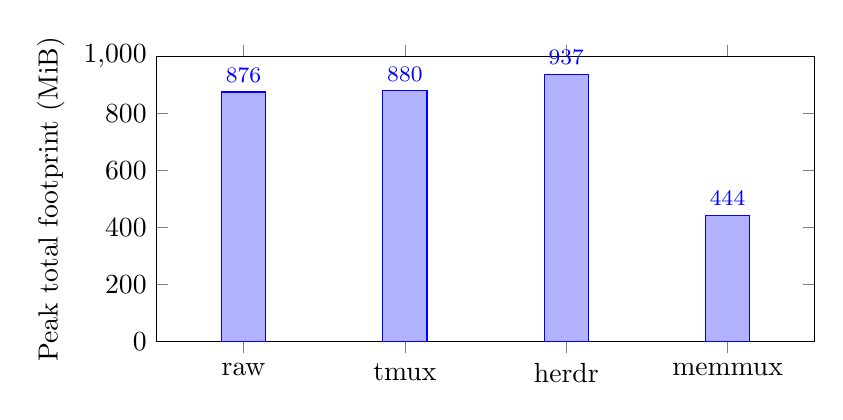
\begin{tikzpicture}
\begin{axis}[
  width=0.82\linewidth, height=5.2cm,
  ybar, bar width=16pt,
  ymin=0, ymax=1000,
  ylabel={Peak total footprint (MiB)},
  symbolic x coords={raw, tmux, herdr, memmux},
  xtick=data, enlarge x limits=0.18,
  nodes near coords, nodes near coords style={font=\footnotesize},
  every axis plot/.append style={fill=teal!30,draw=teal!60!black},
]
\addplot coordinates {(raw,876) (tmux,880) (herdr,937) (memmux,444)};
\draw[dashed,thick,red!70!black] (axis cs:raw,3000) -- (axis cs:memmux,3000);
\end{axis}
\end{tikzpicture}
\caption{Peak footprint of a four-agent fleet under a 3000\,MiB budget (\emph{overcommit}, $N{=}4$).
\sys{} governs by deferring admissions; the others are ungoverned. (The budget line sits above the
plotted range; no launcher approached it because the stub's real RSS is far below the reserved
peak---see Section~\ref{sec:limits}.)}
\label{fig:h4}
\end{figure}

The \emph{no-lost-work} half of H4 is a capability we verify but did not trigger in these runs:
because \sys{} defers at admission, the pressure ladder rarely needs to reclaim a running victim.
A daemon-level test confirms the guarantee directly---a task with a dirty Git worktree, forced into
the emergency stage, produces a checkpoint carrying its patch hash \emph{before} the process is
terminated. The ungoverned launchers have no checkpoint mechanism, so this too is reported as a
capability they lack rather than a number.

\subsection{H1 and H5: attribution and overhead}

Across every run, \sys{} attributed 100\% of each launched tree's proportional memory to its owning
task (H1); the managed-set framing makes this the meaningful figure rather than a host-wide ratio.
The cost of governance is real and we report it plainly (Table~\ref{tab:cost}): \sys{}'s daemon adds
a manager-memory overhead between \code{tmux}'s and \code{herdr}'s, and its steady-state CPU is a
small single-digit percentage. The $\leq 2\%$ CPU target (H5) is defined at a 20-agent fleet; our
small-$N$ measurement is noisy and we do not claim to have met it here---establishing it at scale is
part of the Linux reference run.

\begin{table}[t]
\centering\small
\begin{tabular}{@{}lrr@{}}
\toprule
Launcher & Manager overhead (MiB) & Manager CPU \\
\midrule
raw-baseline & 0.0            & --- \\
tmux 3.6a    & $6.6\pm1.0$    & 0.00\% \\
herdr 0.8.0  & $35.4\pm0.7$   & 0.22\% \\
\sys{} 0.8.0 & $23.1\pm3.4$   & $\sim$2.0\% \\
\bottomrule
\end{tabular}
\caption{The cost of governance (\emph{burst}, $N{=}2$, 3 trials, mean\,$\pm$\,95\% CI). Manager
overhead is the multiplexer's own resident memory, separate from the agents it hosts.}
\label{tab:cost}
\end{table}

\section{Discussion and Limitations}
\label{sec:limits}

\paragraph{One host, one OS.} Every number is from a single macOS machine. macOS does not expose
per-process swap or USS, so the swap-thrashing story---the sharpest version of H4, where an
ungoverned fleet drives the machine onto the swap cliff---cannot be shown here. That measurement is
Linux-specific and is the first item on the reference run.

\paragraph{Stub, not a live agent.} We trade realism for reproducibility and fairness: identical
deterministic workloads across launchers. Real coding agents have burstier, larger, and correlated
footprints; the qualitative guarantees (attribution, cleanup, escape visibility, admission) do not
depend on the workload, but the specific megabytes will differ.

\paragraph{Conservative admission.} \sys{} reserves each task's \emph{class-predicted peak}, which
for our stub is far above its actual RSS. This is why the fleet in Figure~\ref{fig:h4} sits well
under budget: admission is protecting against the reservation, not the live footprint. An
EWMA-refined predictor that tightens reservations toward observed peaks is designed and is future
work; until then \sys{} is safe but leaves headroom on the table.

\paragraph{Modest scale.} We report $N \leq 4$. The harness sweeps $N \in \{1,5,10,20\}$ and the
reproducer emits the footprint-versus-$N$ curve; we simply have not run the full sweep on a machine
where the larger fleets are meaningful.

\paragraph{Empirical, not formal.} These are runtime monitors with measured pass/fail behavior, not
machine-checked proofs. We claim the signals are \emph{checkable and checked}, not that the engine is
formally verified.

\section{Reproducibility}
\label{sec:repro}

\sys{} and its benchmark are open source (MIT). A single command,
\code{memmux-bench paper}, runs the full matrix---every launcher, scenario, and fleet size, with
repeated trials---captures the host specification (\code{host.json}), and regenerates every table and
figure in this paper plus the raw per-sample and per-process JSON Lines time series. Competitor
versions and the measurement date are embedded in the generated report, and any launcher that could
not be driven on the host is listed with its reason. Reproducing the evaluation on a Linux reference
machine is therefore one invocation.

\section{Ethics and Responsible Use}

\sys{} is defensive infrastructure: it makes a developer's own machine account for, and protect, the
work of the agents that developer is running. Its most consequential action---terminating an agent
under memory pressure---is gated on first persisting that agent's uncommitted work, so the failure
mode is a recoverable checkpoint rather than lost effort. We see no dual-use concern beyond that of
any process supervisor.

\section{Conclusion}

Fleets of coding agents have outrun the tools we use to run them. Multiplexers arrange them; nothing
governs them. We argued that memory governance for such fleets is a verification problem and built
\sys{} to make five concrete guarantees checkable at runtime, together with a benchmark honest enough
to admit where those guarantees do \emph{not} distinguish us. The preliminary numbers already show a
clear separation from an ungoverned baseline and a capability---seeing and containing what escapes---
that the alternatives structurally lack. The path from here is a Linux reference run at fleet scale
and a live-agent workload; the reproducer makes both a single command away.

\small
\bibliographystyle{plainnat}
\bibliography{refs}

\normalsize
\appendix
\section{Reproducer invocation}
The canonical run and a fast smoke run:
\begin{verbatim}
memmux-bench paper --out paper-out
memmux-bench paper --agents-sweep 1,2 --scenarios hold \
    --trials 1 --max-samples 3 --agent-budget-mib 3000 --out /tmp/smoke
\end{verbatim}
Each writes \code{host.json}, \code{report.md}, per-cell \code{*.jsonl} and \code{*.procs.jsonl}
time series, and the SVG figures. The host specification block of the generated report records OS,
architecture, physical RAM, CPU model, core count, and tool versions.

\end{document}
